\begin{frame}[fragile]
  \frametitle{Chare Array: Hello Example }
  \lstinputlisting{code/arrayHello.ci}
\end{frame}

\begin{frame}[fragile]
  \frametitle{Chare Array: Hello Example }
  \lstinputlisting[basicstyle=\scriptsize]{code/arrayHello.cpp}
\end{frame}

\begin{frame}[fragile]
   \frametitle{Hello World Array Projections Timeline View}\scriptsize
  \begin{itemize}
    \item Add \texttt{-tracemode projections} to link line to enable tracing
    \item Run Projections tool to load trace log files and visualize performance
  \end{itemize}
  \begin{center} 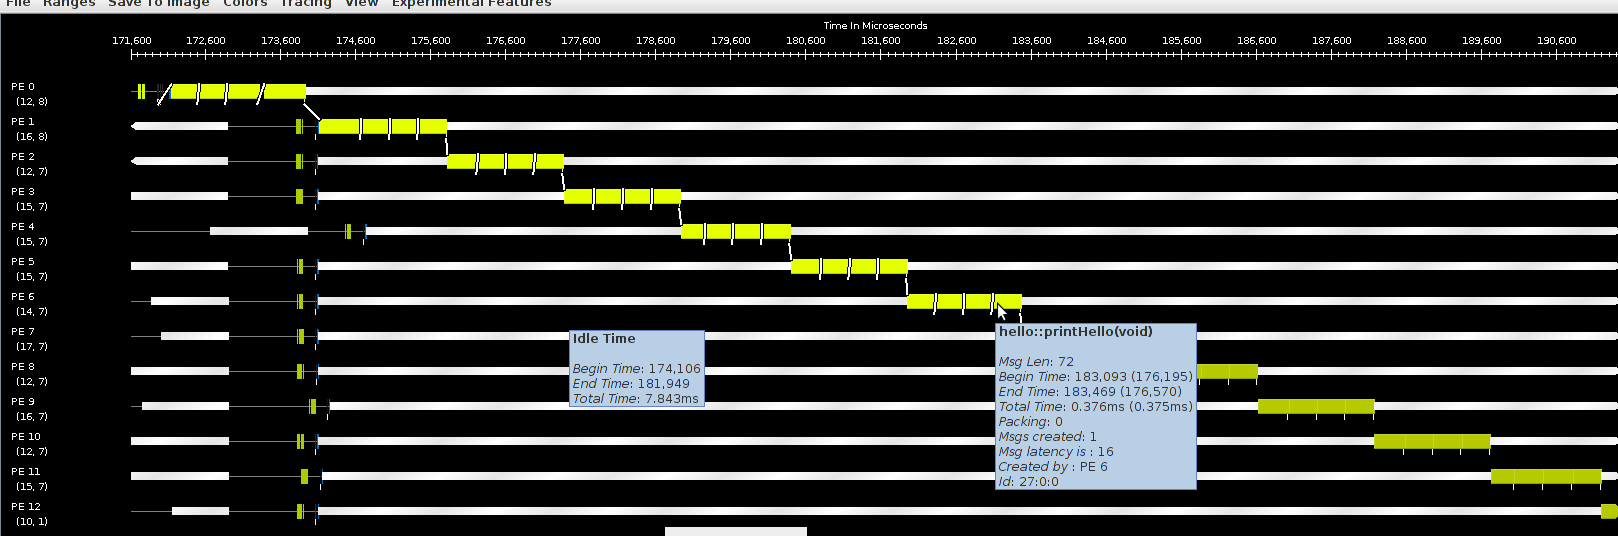
\includegraphics[width=0.99\textwidth]{figures/arrayHelloTimeline} \end{center}
  \begin{itemize}
   \item arrayHello on BG/Q 16 Nodes, mode c16, 1024 elements (4 per process)
  \end{itemize}
\end{frame}


